\documentclass[tikz,border=8pt]{standalone}
% Shared look for every TikZ diagram. Load with \input{../../tools/tikz-style.tex}
\usepackage[T1]{fontenc}
\usepackage{lmodern}
\renewcommand{\sfdefault}{lmr}  % diagrams use the same serif as the text
\usetikzlibrary{arrows.meta, positioning, shapes.geometric, calc, fit, backgrounds}
\definecolor{cblue}{HTML}{4C78A8}
\definecolor{corange}{HTML}{F58518}
\definecolor{cgreen}{HTML}{54A24B}
\definecolor{cred}{HTML}{E45756}
\definecolor{cpurple}{HTML}{B279A2}
\definecolor{cgrey}{HTML}{6B6B6B}
\tikzset{
  every picture/.style={font=\sffamily, line width=1.2pt},
  box/.style={draw=#1, fill=#1!12, rounded corners=4pt, align=center, inner sep=7pt, minimum height=1.1cm},
  box/.default=cgrey,
  arrow/.style={-{Stealth[length=3mm]}, draw=cgrey, line width=1.4pt},
  title/.style={font=\sffamily\bfseries\Large},
  note/.style={font=\sffamily\small, text=cgrey, align=center},
}
\AtBeginDocument{\hyphenpenalty=10000 \exhyphenpenalty=10000}

% The green pole relative to the robot: dx = -1.6, dy = 1.2. arctan(dy/dx) = arctan(-0.75) = -36.87 deg points
% down-right, the wrong side. atan2(1.2, -1.6) = 143.13 deg points up-left, at the pole.
\begin{document}
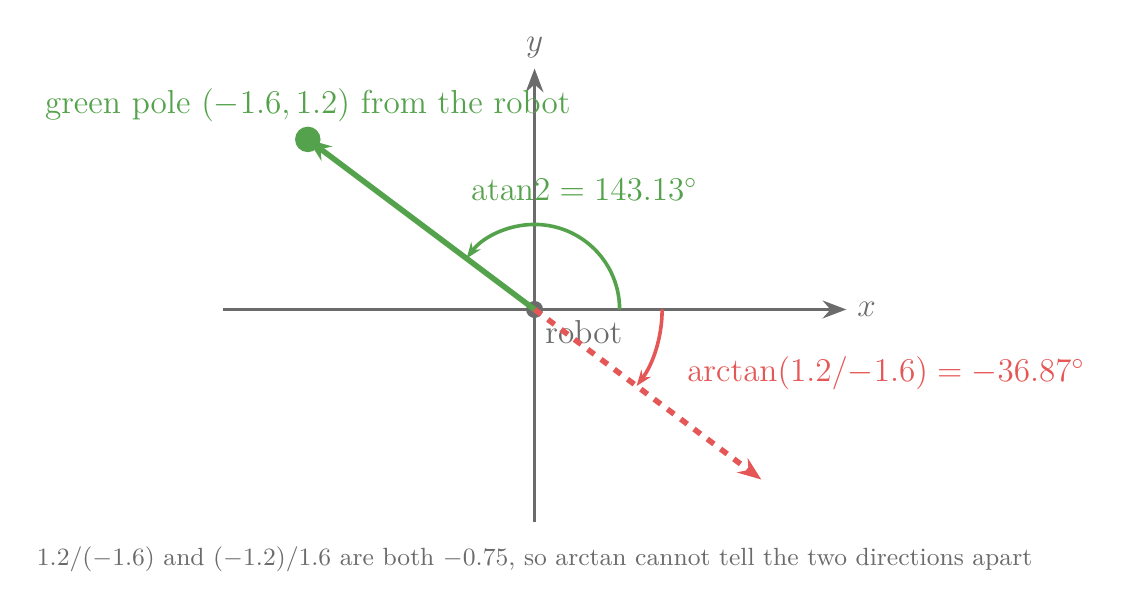
\begin{tikzpicture}[scale=1.8, every node/.append style={font=\large}]
  \draw[cgrey, -{Stealth[length=3mm]}] (-2.2,0) -- (2.2,0) node[right] {$x$};
  \draw[cgrey, -{Stealth[length=3mm]}] (0,-1.5) -- (0,1.7) node[above] {$y$};
  \fill[cgrey] (0,0) circle (0.06); \node[below right, cgrey] at (0,0) {robot};
  \fill[cgreen] (-1.6,1.2) circle (0.09);
  \node[cgreen, above] at (-1.6,1.25) {green pole $(-1.6, 1.2)$ from the robot};
  \draw[cgreen, line width=2pt, -{Stealth[length=3mm]}] (0,0) -- (-1.6,1.2);
  \draw[cgreen, line width=1.3pt, -{Stealth[length=2mm]}] (0.6,0) arc (0:143.13:0.6);
  \node[cgreen] at (0.35,0.85) {$\mathrm{atan2} = 143.13^\circ$};
  \draw[cred, line width=2pt, dashed, -{Stealth[length=3mm]}] (0,0) -- (1.6,-1.2);
  \draw[cred, line width=1.3pt, -{Stealth[length=2mm]}] (0.9,0) arc (0:-36.87:0.9);
  \node[cred, right] at (1.0,-0.45) {$\arctan(1.2 / {-1.6}) = -36.87^\circ$};
  \node[note, anchor=north] at (0,-1.6) {$1.2 / (-1.6)$ and $(-1.2) / 1.6$ are both $-0.75$, so arctan cannot tell the two directions apart};
\end{tikzpicture}
\end{document}
